% ======================================================================
%  Tunable gel-point positioning in 3D percolation networks
%  Physical Review Letters — REVTeX 4.2, two-column
%  Fallback journal: Physical Review E (same content, relaxed length)
% ======================================================================
\documentclass[aps,prl,twocolumn,superscriptaddress,floatfix,nofootinbib,longbibliography]{revtex4-2}

\usepackage{graphicx}
\usepackage{amsmath,amssymb}
\usepackage{bm}
\usepackage{booktabs}
\usepackage[colorlinks=true,allcolors=blue]{hyperref}

\graphicspath{{figures_v2/}{paper_drafts/figures_v2/}{./}}

% convenience macros
\newcommand{\msd}{\langle r^2(t)\rangle}
\newcommand{\pc}{p_c}
\newcommand{\pcp}{p_c'}
\newcommand{\kap}{\kappa}
\newcommand{\nueff}{\nu_{\mathrm{eff}}}

\begin{document}

\title{Nucleation density programs the viscoelastic gel point of a percolation network}

\author{A.~Author}
\author{B.~Author}
\author{C.~Author}
\author{D.~Author}
\affiliation{[Affiliation], [Institution], [City], [Country]}

\date{\today}

\begin{abstract}
Passive microrheology locates the viscoelastic gel point through the Winter--Chambon condition $\alpha=0.5$. Using three-dimensional random walks in the void of site-percolation lattices, we show that this dynamical gel point agrees, to within the $p$-grid, with the purely geometric void-spanning threshold for nucleation densities $\kap\lesssim0.8$. At $\kap=0$ that common value is $\pcp(\infty)\approx0.681$, about one percent below the Bernoulli void threshold $1-\pc=0.6884$. A single nucleation-density parameter $\kap$ then shifts both thresholds from this anchor toward unity. They part only as growth becomes compact, where passive microrheology mildly over-reads the structural gel point. Data collapse gives an effective exponent $\nueff\approx1.6$ with no systematic $\kap$ trend for $\kap\le0.8$, distinct from the static percolation value $\nu=0.88$.
\end{abstract}

\maketitle

% ===================== MAIN LETTER =====================
Gelation---the transition of a polymer solution or colloidal suspension from a viscous fluid to a viscoelastic solid---is characterized by a gel point $\pcp$ at which the loss tangent $\tan\delta = G''/G'$ becomes frequency independent and equal to unity~\cite{Chambon1987,Winter1987}. In the Winter--Chambon picture this is the phase angle $\delta=45^{\circ}$ and a power-law mean squared displacement (MSD) $\msd\propto t^{0.5}$, both accessible by passive microrheology through the Generalized Stokes--Einstein Relation (GSER)~\cite{Mason1995,Mason2000,Squires2010fluid}. The gel point is routinely treated as a fixed property of composition---set by concentration, cross-link density, and temperature~\cite{Rubinstein2003,Larson1999}. What is rarely asked is whether it also depends on \emph{how} the network forms: on the spatial growth dynamics of the cluster itself, which in real colloidal and biopolymer gels range from open fractal aggregates to compact space-filling domains~\cite{Trappe2001,Coniglio2004,Ng2008}.

Larsen and Furst located that point in a crosslinking hydrogel by particle-tracking microrheology and the Winter--Chambon criterion~\cite{Larsen2008,Corrigan2009}. That is the measurement precedent: passive microrheology already reads the gel point of a real gel. The mechanism precedent is growth-rule percolation. Changing the rule by which a cluster is assembled shifts the percolation threshold and can change the order of the transition, at fixed composition~\cite{Anderson1988,Roy2017,Roy2018,DSouzaNagler2015}. Neither line identifies the passive-microrheology gel point with void spanning and then moves it by one nucleation density. That is the gap this Letter fills.

Probe particles diffuse through the \emph{void} (fluid) phase of the network, not through the network~\cite{deBruyn2013,Rich2011,Oppong2006}. We place random walkers on the unoccupied sublattice of an $L\times L\times L$ simple cubic lattice, sweep the occupation probability $p$, and extract the anomalous-diffusion exponent $\alpha(p)$ from $\msd\propto t^{\alpha}$ over the intermediate window $[L_W/100,L_W/10]$. The gel point is the occupation at which $\alpha=0.5$, equivalently $\delta=45^{\circ}$ for a power-law MSD through the GSER~\cite{Winter1987,Chambon1987,Muthukumar1989}. Walkers move to a uniformly chosen nearest neighbor if it is unoccupied and otherwise dwell for a short binding time; the ensemble MSD is accumulated online. The finite-size protocol and the walk-dimension argument for $\alpha\approx0.5$ are given in the End Matter. The GSER spectra, the full $\kap$ table, and the code notes are in the Supplemental Material~\cite{SM}.

Network growth is controlled by a nucleation-density parameter $\kap\in[0,1]$. At each increment in $p$, a fraction $(1-\kap)$ of the newly occupied sites are placed as independent random nuclei and the remainder are grown by nearest-neighbor adjacency from the existing cluster frontier. Thus $\kap=0$ is classical Bernoulli site percolation (every site an independent seed: maximal nucleation density), $\kap=1$ is single-seed compact (Eden~\cite{Eden1961}) growth, and intermediate $\kap$ interpolates between a spatially uniform obstacle field and a compact, clustered network. The seed fraction $1-\kap$ is the nucleation density---independent nuclei per newly occupied site---so $\kap$ indexes that density inversely. We treat $\kap$ as a coarse-grained proxy for nucleation conditions that are varied experimentally through cross-linker concentration, thermal-ramp rate, or ionic strength, rather than a parameter set directly in the laboratory.

\emph{The gel point is the void-percolation transition.}---For random growth ($\kap=0$), $\alpha(p)$ falls from Fickian diffusion ($\alpha\approx1$) through the gel criterion and arrests sharply [Fig.~\ref{fig:random}]. The crossing is essentially size independent above $L=200$, extrapolating to
\begin{equation}
  \pcp(\infty)\approx0.681 ,
\end{equation}
about one percent below the complementary void-percolation threshold $1-\pc=0.6884$ ($\pc=0.3116$). Walkers occupy the void sublattice, which loses spanning connectivity at $p=1-\pc$, where the incipient cluster gives $\msd\propto t^{0.5}$. On the same lattices the geometric void-spanning threshold $\pcp^{\mathrm{geom}}$ agrees with the dynamical gel point $\pcp^{\mathrm{MR}}$ (the $\alpha=0.5$ crossing) to within the $p$-grid for $\kap\lesssim0.8$ [Fig.~\ref{fig:geom}]. Thus $\pcp\simeq1-\pc$ is the Bernoulli ($\kap=0$) limit of a threshold the two measurements share. The two part only for $\kap\gtrsim0.85$, as the void compactifies into large finite pockets: there $\pcp^{\mathrm{MR}}>\pcp^{\mathrm{geom}}$, so passive microrheology mildly over-reads the structural gel point, reporting gelation at higher occupancy than the loss of connectivity.

\emph{Nucleation density tunes the gel point.}---Increasing $\kap$ (lowering the nucleation density) shifts the $\alpha=0.5$ crossing monotonically to higher $p$ [Fig.~\ref{fig:tuning}]. A compact, connected cluster of a given mass occupies a more localized region than the same number of randomly placed sites, leaving a larger and better-connected void that percolates only at higher occupation. Finite-size scaling gives thermodynamic gel points rising smoothly with $\kap$: $\pcp(\infty)=0.681,\,0.702,\,0.722$ for $\kap=0,\,0.6,\,0.8$, resolved cleanly, rising to $\pcp(\infty)\approx0.79$--$0.80$ at $\kap=0.97$---a broadened crossover point carrying larger uncertainty (see below)---and continuing toward the single-seed Eden limit, where a single compact cluster can fill the lattice before fragmenting the void ($\pcp\to1$, treated as an asymptotic bound rather than a finite critical point). A fine $\kap$-grid at fixed $L$ resolves the full curve $\pcp(\kap)$~\cite{SM}, monotonic with two regimes separated near a $\sim1\%$ seed fraction ($\kap\approx0.99$): a gradual rise where many nuclei keep the morphology quasi-random, and a steep rise toward unity where single-cluster growth dominates. Across the accessible range the gel point spans $\pcp\approx0.68$--$0.91$, approaching unity only asymptotically in the Eden limit.

\emph{No $\kap$ trend in $\nueff$.}---Finite-size scaling across $L=50$--$750$ asks whether moving $\pcp$ with $\kap$ changes the character of the transition. The gel point converges by $L\approx200$, so the shift $\pcp(L)=\pcp(\infty)+aL^{-1/\nu}$ fixes $\pcp(\infty)$ but leaves $\nu$ underdetermined. The exponent comes from the data collapse of $\alpha(p,L)$ and, separately, from the transition width $w(L)\sim L^{-1/\nu}$ [Fig.~\ref{fig:fss}]. Collapse gives $\nueff=1.62$, $1.64$, and $1.67$ at $\kap=0$, $0.6$, and $0.8$, with no systematic $\kap$ trend. The width estimator agrees at $\kap=0$ ($1.77\pm0.21$) and $\kap=0.8$ ($1.69\pm0.03$) and is lower at $\kap=0.6$ ($1.49\pm0.05$). Conditions with $\kap\ge0.97$ lie in the Eden crossover, where the estimators become unreliable, and are excluded (End Matter). This effective exponent differs from the static 3D site-percolation value $\nu=0.88$, because $\pcp$ is defined through the probe-diffusion exponent: the width over which $\alpha$ crosses $0.5$ need not scale with the static correlation length.

Because the MSD is a power law over the anomalous window, the GSER yields $G',G''\propto\omega^{\alpha}$ with a frequency-independent phase angle $\delta=90\alpha$ in degrees; at $\pcp$ this is $G'\approx G''$ and $\delta\approx45^{\circ}$ at each shifted gel point~\cite{SM}.

The gel point read by passive microrheology is the void-spanning threshold, one nucleation density moves that threshold from the Bernoulli anchor toward unity, and the transition has a single effective exponent $\nueff\approx1.6$ with no systematic $\kap$ trend for $\kap\le0.8$. Whether $\nueff$ takes an exact value remains open.

\begin{acknowledgments}
[Acknowledgments to be completed.]
\end{acknowledgments}

\section*{Data availability}
The $\alpha(p,L)$ tables, the finite-size fits, and the ensemble mean-squared-displacement curves will be deposited as CSV files at Zenodo, and this statement will cite that deposit by DOI at publication. Occupied-site configurations will be included in the same deposit as logical vectors, with the reshape that recovers the cubic lattice. Code that generates the walks is described in the Supplemental Material~\cite{SM} and will be deposited with the data.

% ---------------- main-text figures ----------------
\begin{figure}[t]
  \centering
  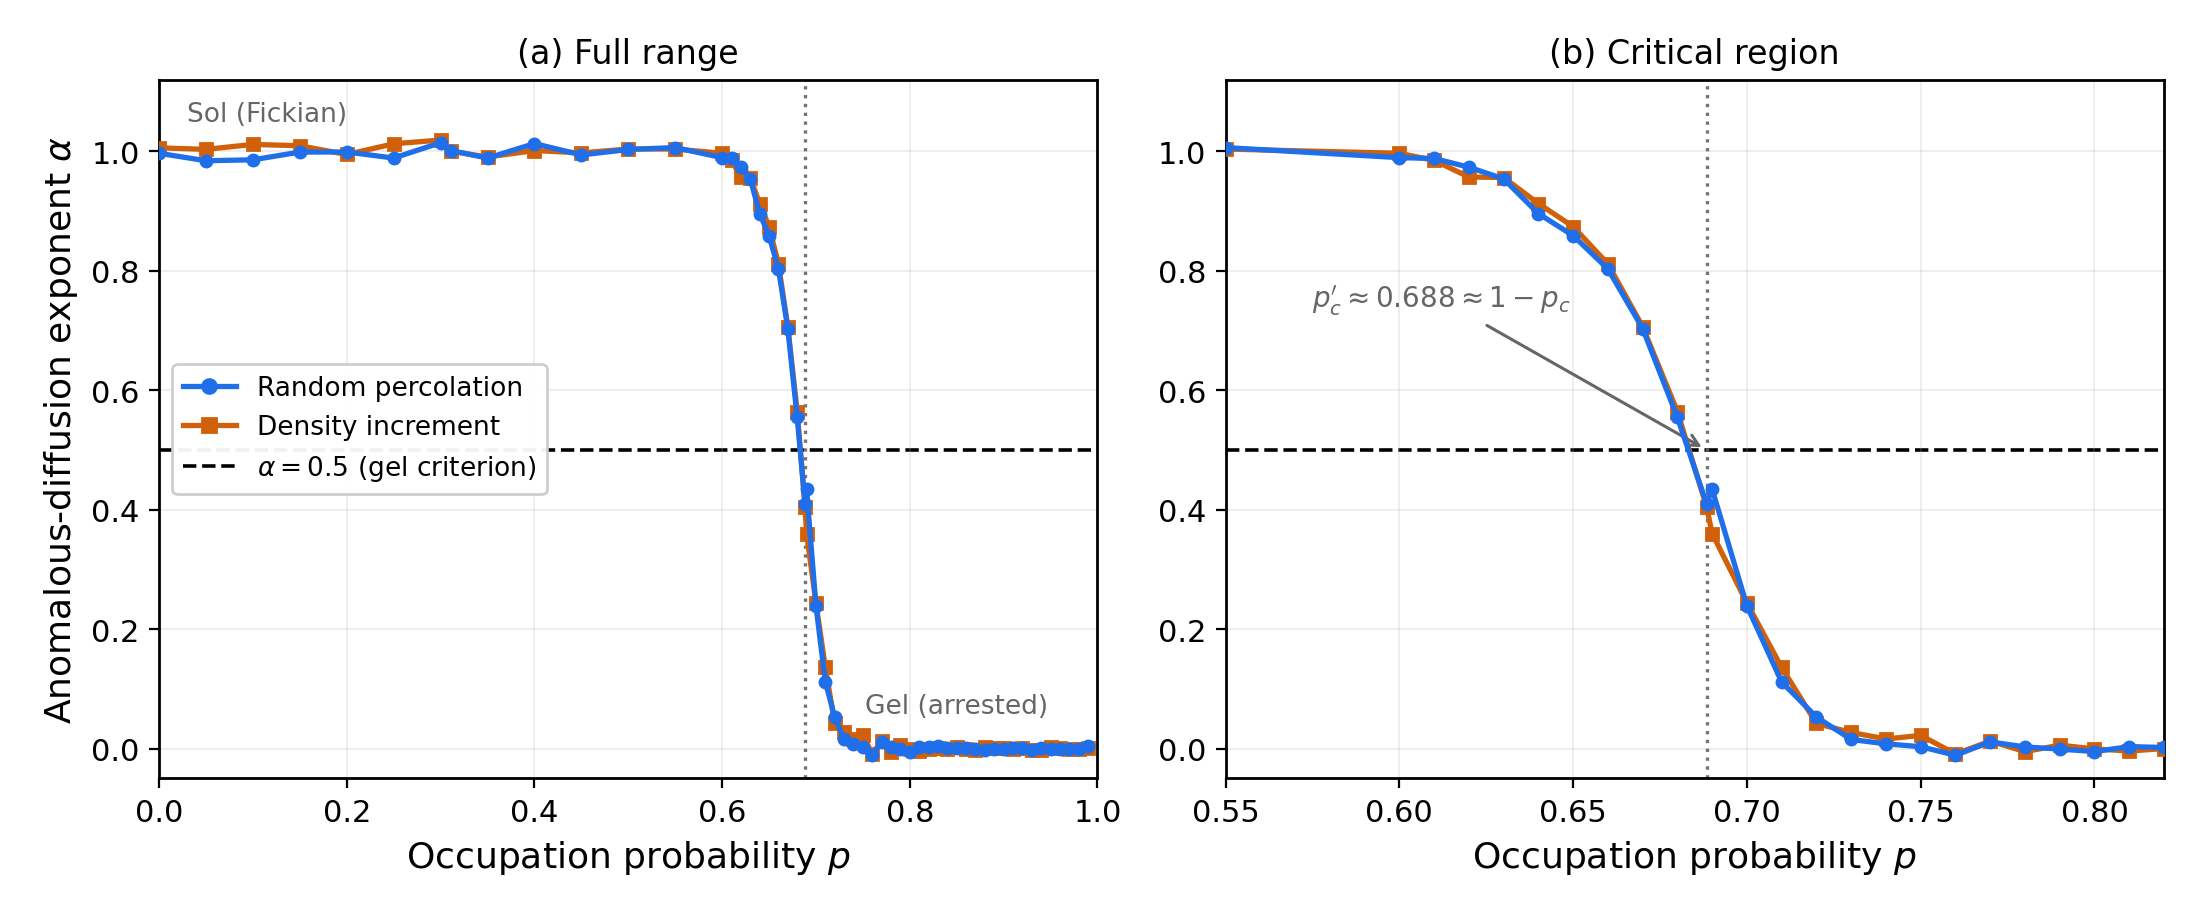
\includegraphics[width=\linewidth]{fig1_random_alpha_vs_p.png}
  \caption{\textbf{The gel point is the void-percolation transition.}
    Anomalous-diffusion exponent $\alpha(p)$ for random ($\kap=0$) growth:
    Fickian diffusion ($\alpha\approx1$) gives way, through the Winter--Chambon
    criterion $\alpha=0.5$ (dashed), to arrest. Finite-size scaling places the
    gel point at $\pcp(\infty)\approx0.681$, about one percent below the
    void-percolation threshold $1-\pc=0.6884$ ($\pc=0.3116$).}
  \label{fig:random}
\end{figure}

\begin{figure*}[t]
  \centering
  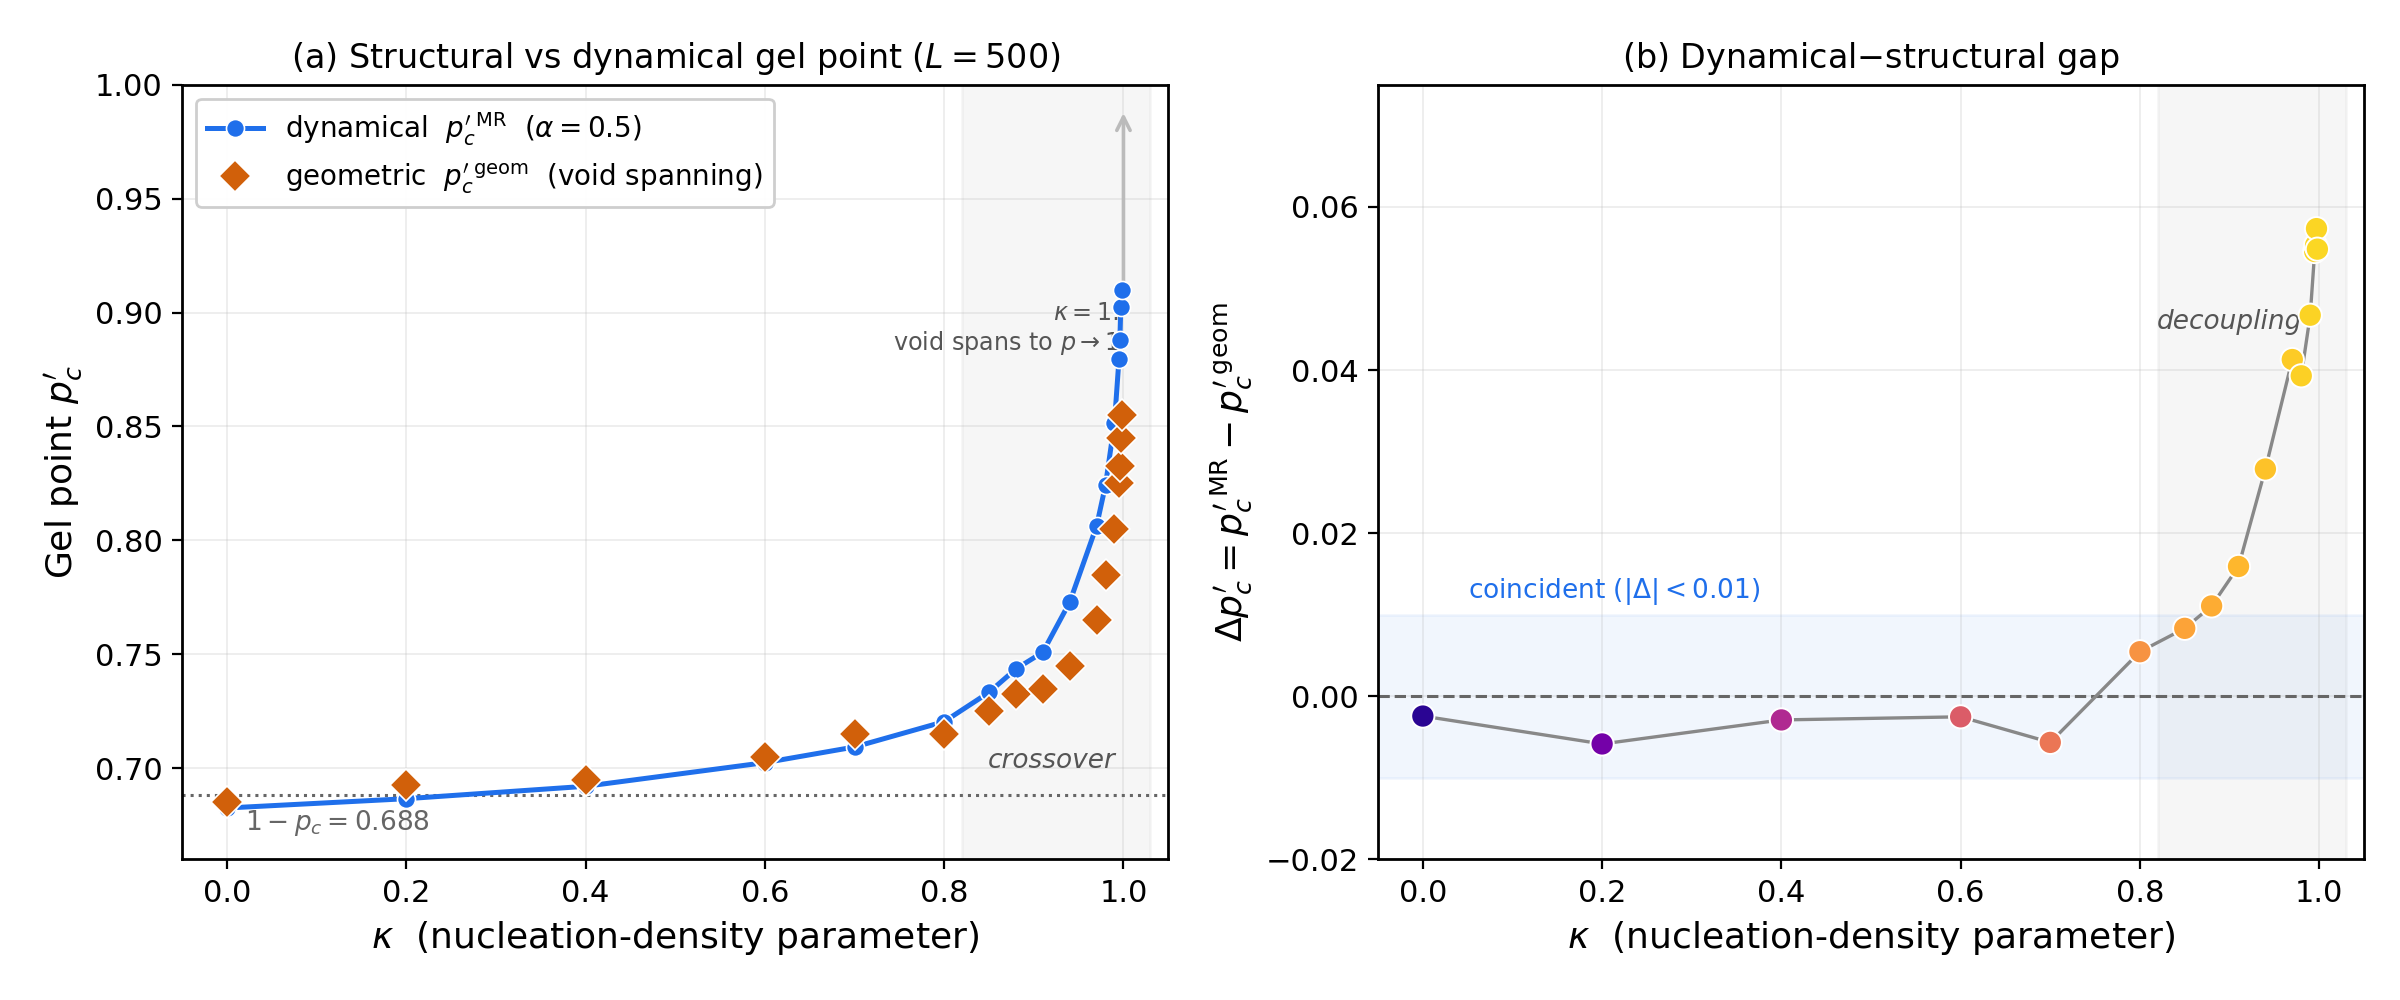
\includegraphics[width=\linewidth]{fig_dyn_vs_geom.png}
  \caption{\textbf{The microrheological gel point tracks the void-spanning threshold.}
    (a) Dynamical gel point $\pcp^{\mathrm{MR}}$ (the $\alpha=0.5$ crossing) and the geometric
    void-spanning threshold $\pcp^{\mathrm{geom}}$ (loss of a face-to-face spanning empty cluster),
    both at $L=500$. (b) Their difference $\Delta\pcp=\pcp^{\mathrm{MR}}-\pcp^{\mathrm{geom}}$: the
    two agree to within the $p$-grid for $\kap\lesssim0.8$ and part through the
    Eden crossover, the dynamical point lagging the structural one. At $\kap=1$ the void of a single
    compact cluster spans until $p\to1$ (no finite-$p$ threshold).}
  \label{fig:geom}
\end{figure*}

\begin{figure*}[t]
  \centering
  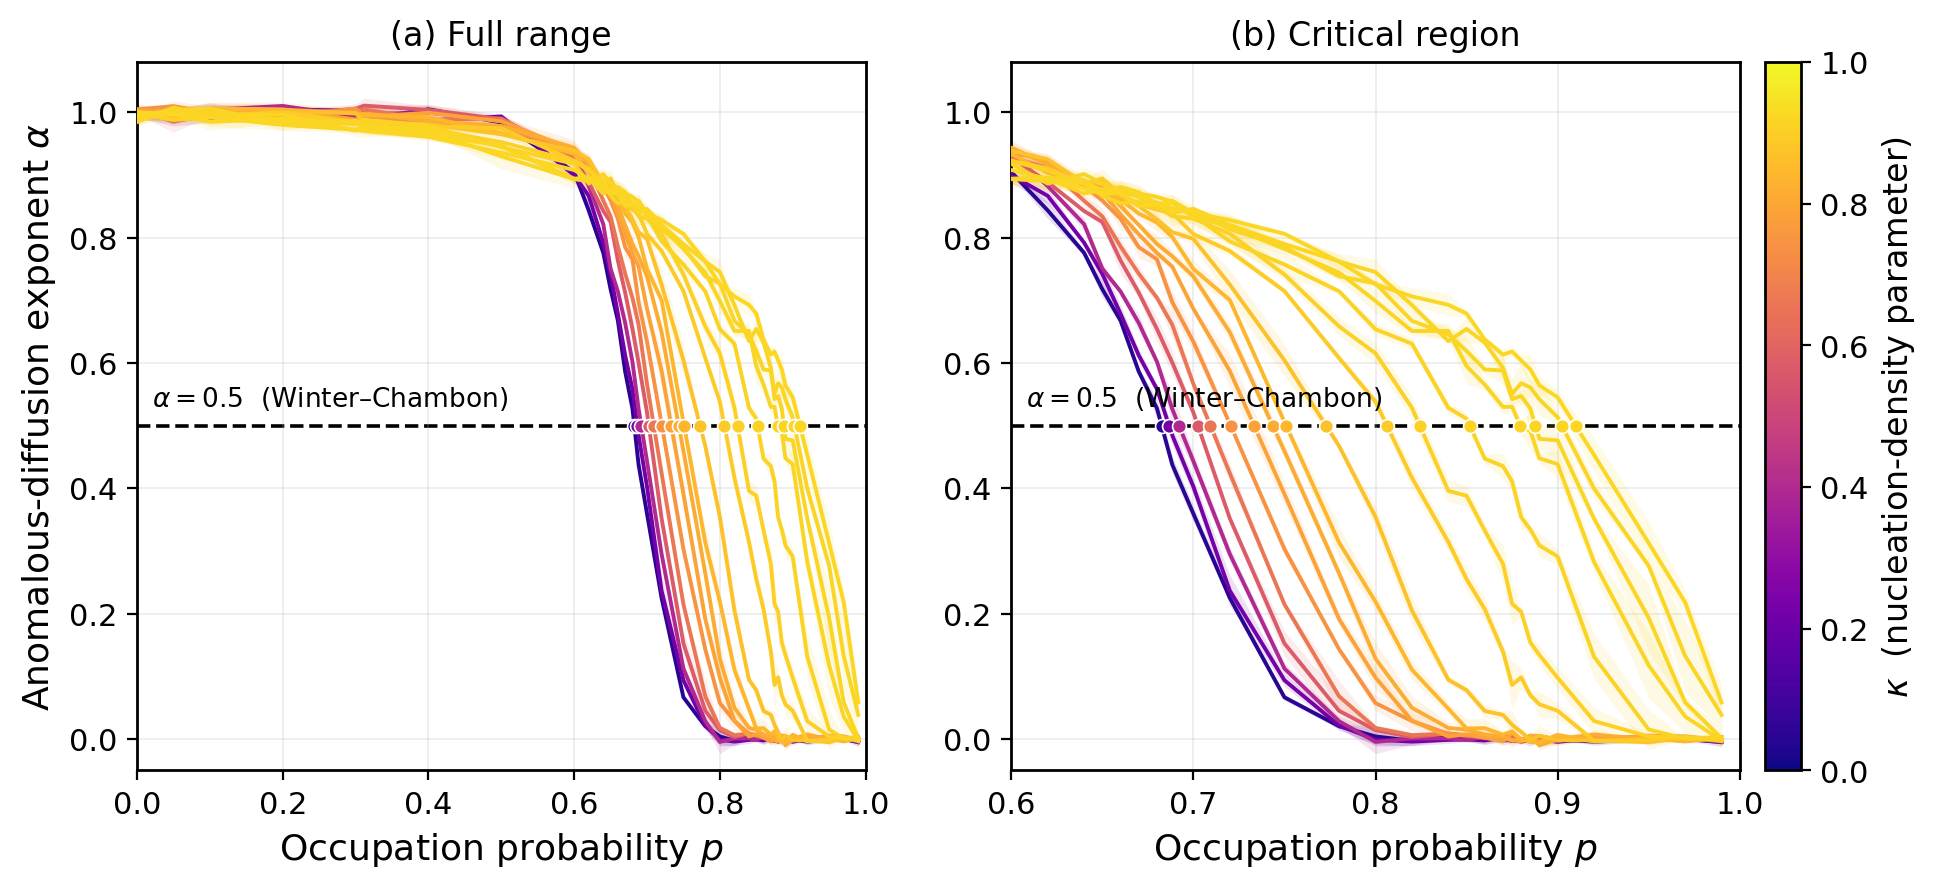
\includegraphics[width=0.48\textwidth]{fig2a_kappa_alpha_vs_p.png}\hfill
  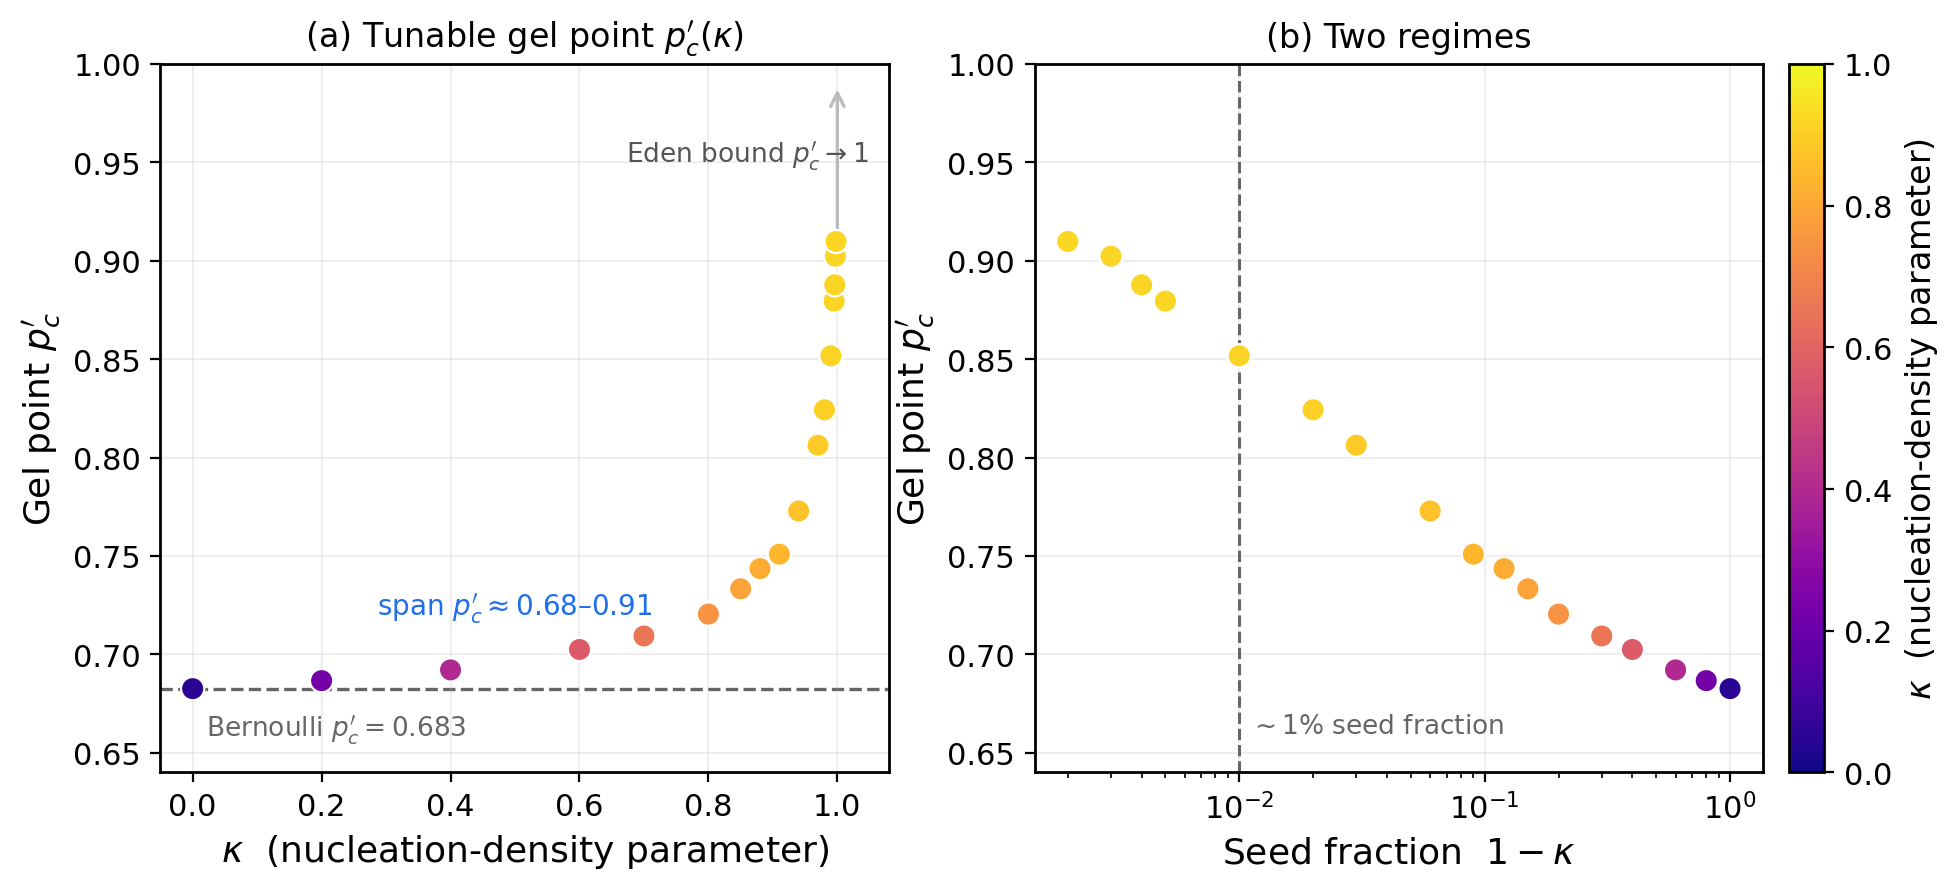
\includegraphics[width=0.48\textwidth]{fig2b_gelpoint_vs_kappa.png}
  \caption{\textbf{Nucleation density tunes the gel point.}
    (a) $\alpha(p,\kap)$: the $\alpha=0.5$ crossing shifts monotonically to
    higher $p$ as $\kap$ increases from $0$ (random) toward $1$ (single-seed
    Eden). (b) Gel-point curve $\pcp(\kap)$, spanning $\pcp\approx0.68$--$0.91$ over the accessible range,
    with two regimes separated near a $\sim1\%$ seed fraction.}
  \label{fig:tuning}
\end{figure*}

\begin{figure*}[t]
  \centering
  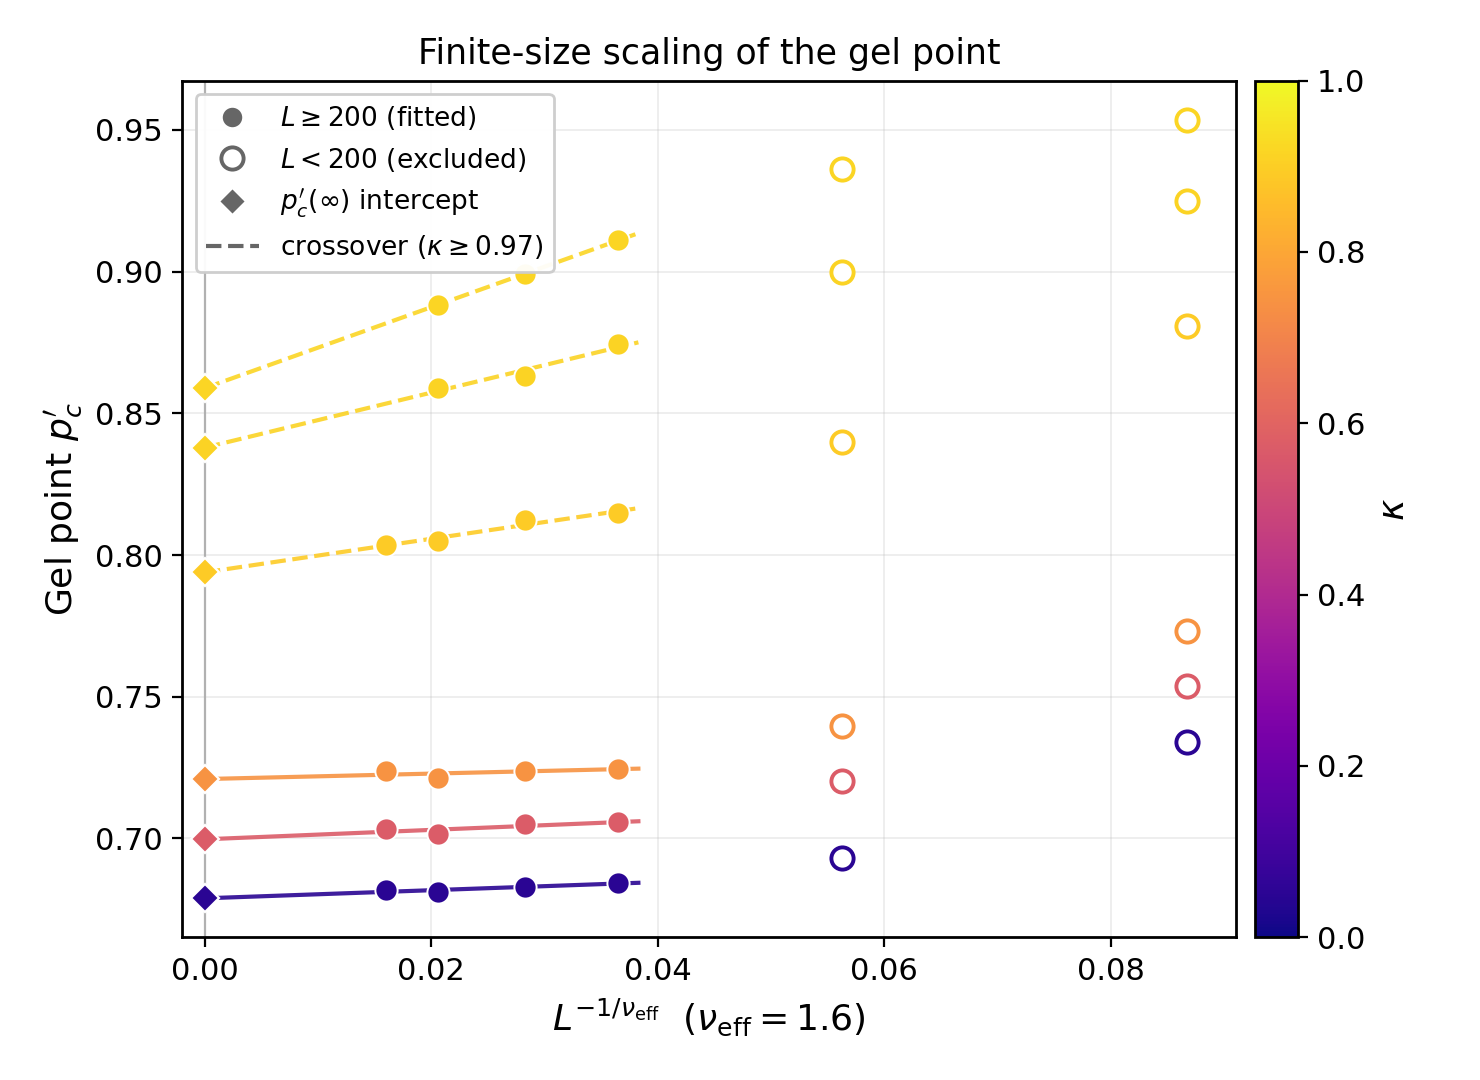
\includegraphics[width=0.48\textwidth]{fig4a_fss_pcL.png}\hfill
  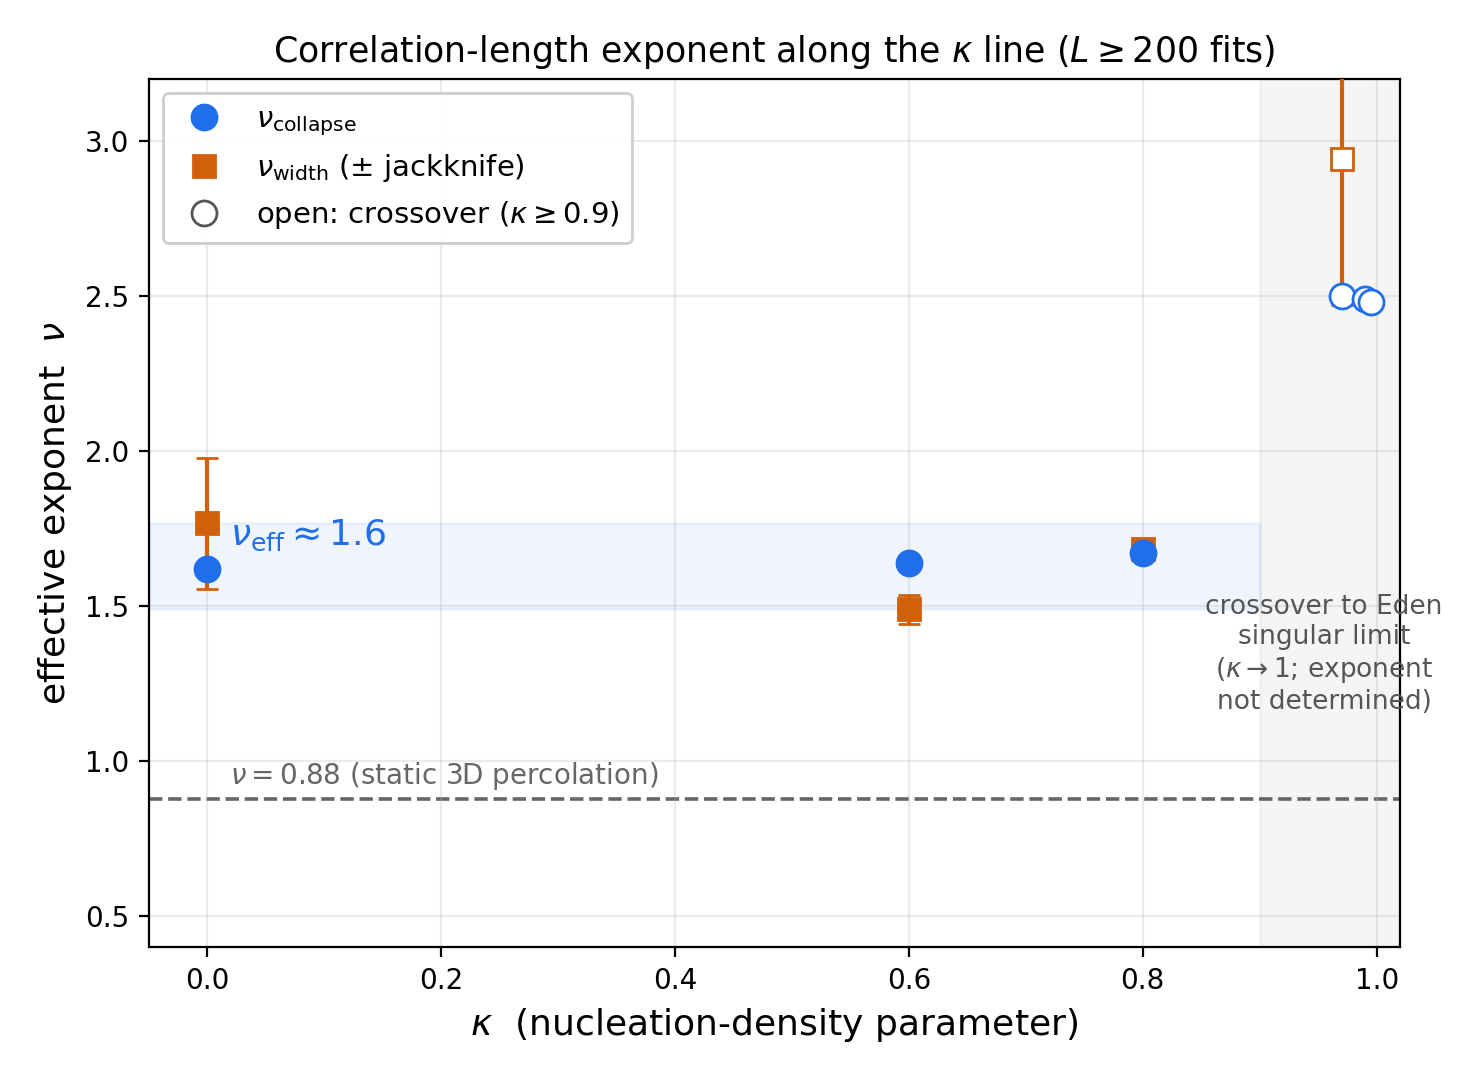
\includegraphics[width=0.48\textwidth]{fig4b_nu_vs_kappa.png}
  \caption{\textbf{Effective exponent of the gel-point transition.}
    (a) Finite-size scaling $\pcp(L)=\pcp(\infty)+aL^{-1/\nu}$ for each $\kap$
    (filled: $L\ge200$ used in fits; open: smaller sizes excluded).
    (b) Effective exponent $\nueff(\kap)$. Collapse gives $\nueff\approx1.6$ with
    no systematic $\kap$ trend for $\kap\le0.8$. The width estimator agrees at
    $\kap=0$ and $0.8$ and is lower at $\kap=0.6$. Both are distinct from static
    3D percolation ($\nu=0.88$, dashed). The $\kap\ge0.97$ points (open) lie in
    the Eden crossover and are excluded.}
  \label{fig:fss}
\end{figure*}

\bibliographystyle{apsrev4-2}
\bibliography{references_enhanced}

% End Matter follows the references and does not count against the core length.
\appendix
\section{Finite-size protocol}
\label{app:fss}
We repeat the analysis at $L\in\{50,100,200,300,500,750\}$ for
$\kap\in\{0,0.6,0.8,0.97,1.0\}$, with two crossover densities
$\kap\in\{0.99,0.995\}$ run to $L\le500$. Because the finite-size crossover
time grows as $L^2$, the steps per walker scale as $L_W(L)=10^6(L/500)^2$, so
the fit window stays inside the anomalous regime at every size. From
$\pcp(L)$ (Table~\ref{tab:pcL}) and the logistic widths $w(L)$ we estimate
$\nu$ three ways: the shift $\pcp(L)=\pcp(\infty)+aL^{-1/\nu}$; the width
$w(L)\sim L^{-1/\nu}$; and the collapse of $\alpha(p,L)$ against
$(p-\pcp(\infty))L^{1/\nu}$, scored by the residual to a master curve in
$\alpha$-space. The sizes $L=50$ and $100$ carry the strongest corrections to
scaling and are excluded from the exponent fits. Uncertainties are by jackknife
over the fitted sizes.

For $L\ge200$, $\pcp(L)$ is already stationary, so the shift fit fixes
$\pcp(\infty)$ and has little leverage on $\nu$. The exponent is taken from
the width and the collapse. Collapse gives $\nueff=1.62$, $1.64$, and $1.67$
at $\kap=0$, $0.6$, and $0.8$ (Table~\ref{tab:nu}), with no systematic $\kap$
trend. The width estimator agrees at $\kap=0$ and $0.8$ and is lower at
$\kap=0.6$ ($1.49\pm0.05$). Beyond $\kap\approx0.9$ the transition crosses over
to the Eden limit: $\pcp(\infty)$ keeps rising
(Table~\ref{tab:pcLcross}), but with only three fit sizes the width and shift
estimators become degenerate and the collapse drifts to $\nu\approx2.5$. We
therefore report $\nueff\approx1.6$ only for $\kap\le0.8$ and treat
$\kap\ge0.97$ as an unresolved crossover. At $\kap=1$ there is no finite-$L$
crossing, and $\pcp\to1$ is a bound.

\begin{table}[h]
\centering
\caption{Size-dependent gel point $\pcp(L)$ and its extrapolation
$\pcp(\infty)$ (shift fit, $L\ge200$).}
\label{tab:pcL}
\begin{tabular}{lcccc}
\toprule
$L$ & $\kap=0$ & $\kap=0.6$ & $\kap=0.8$ & $\kap=0.97$ \\
\midrule
50   & 0.734 & 0.754 & 0.773 & 0.881 \\
100  & 0.693 & 0.720 & 0.740 & 0.840 \\
200  & 0.684 & 0.706 & 0.725 & 0.815 \\
300  & 0.683 & 0.705 & 0.724 & 0.812 \\
500  & 0.681 & 0.702 & 0.721 & 0.805 \\
750  & 0.682 & 0.703 & 0.724 & 0.804 \\
\midrule
$\infty$ & \textbf{0.681} & \textbf{0.702} & \textbf{0.722} & \textbf{$\approx$0.80} \\
\bottomrule
\end{tabular}
\end{table}

\begin{table}[h]
\centering
\caption{Crossover set: $\pcp(L)$ for $\kap=0.99$ and $0.995$, capped at
$L\le500$. The gel point rises toward the Eden bound, but the exponent is not
resolved (Table~\ref{tab:nu}).}
\label{tab:pcLcross}
\begin{tabular}{lcc}
\toprule
$L$ & $\kap=0.99$ & $\kap=0.995$ \\
\midrule
50   & 0.925 & 0.954 \\
100  & 0.900 & 0.936 \\
200  & 0.874 & 0.911 \\
300  & 0.863 & 0.899 \\
500  & 0.859 & 0.888 \\
\midrule
$\infty$ & \textbf{0.857} & \textbf{0.866} \\
\bottomrule
\end{tabular}
\end{table}

\begin{table}[h]
\centering
\caption{Effective exponent from data collapse and from the transition width
($L\ge200$; jackknife uncertainties). Rows with $\kap\ge0.97$ are unresolved
crossover points and are excluded from the reported $\nueff$. ``deg.'' marks a
degenerate few-size fit.}
\label{tab:nu}
\begin{tabular}{lcc}
\toprule
$\kap$ & $\nu$ (collapse) & $\nu$ (width) \\
\midrule
0.0  & 1.62 & $1.77\pm0.21$ \\
0.6  & 1.64 & $1.49\pm0.05$ \\
0.8  & 1.67 & $1.69\pm0.03$ \\
0.97  & 2.50 & $2.94\pm0.47$ \\
0.99  & 2.49 & deg. \\
0.995 & 2.48 & deg. \\
\bottomrule
\end{tabular}
\end{table}

\section{Walk dimension of the critical void}
\label{app:dw}
At the void-percolation threshold the probe explores a critical, fractal void,
so its diffusion is anomalous, $\msd\propto t^{2/d_w}$, with $d_w$ the walk
dimension of the incipient cluster~\cite{Gefen1983,Havlin1983,Straley1980,Argyrakis1985}.
For three-dimensional lattice percolation $d_w=3.88(3)$~\cite{Kammerer2008}, so
$2/d_w=0.515(4)$, within one percent of the Winter--Chambon value $\alpha=0.5$.
The gel criterion and the percolation threshold therefore meet because the
three-dimensional walk exponent lies close to $0.5$. The match is specific to
three dimensions: in two dimensions $d_w=2.878(1)$ gives $2/d_w=0.70$, far
from $0.5$. This fixes the random ($\kap=0$) anchor, where the void at
$p=1-\pc$ is itself a critical Bernoulli configuration~\cite{AlexanderOrbach1982}.
Continuum void percolation has a larger walk dimension~\cite{Kammerer2008}; the
lattice model here is in the lattice-percolation class, for which
$2/d_w\approx0.52$.

\end{document}
